\section{moeo\-One\-Objective\-Comparator$<$ MOEOT $>$ Class Template Reference}
\label{classmoeoOneObjectiveComparator}\index{moeoOneObjectiveComparator@{moeoOneObjectiveComparator}}
Functor allowing to compare two solutions according to one objective.  


{\tt \#include $<$moeo\-Comparator.h$>$}

Inheritance diagram for moeo\-One\-Objective\-Comparator$<$ MOEOT $>$::\begin{figure}[H]
\begin{center}
\leavevmode
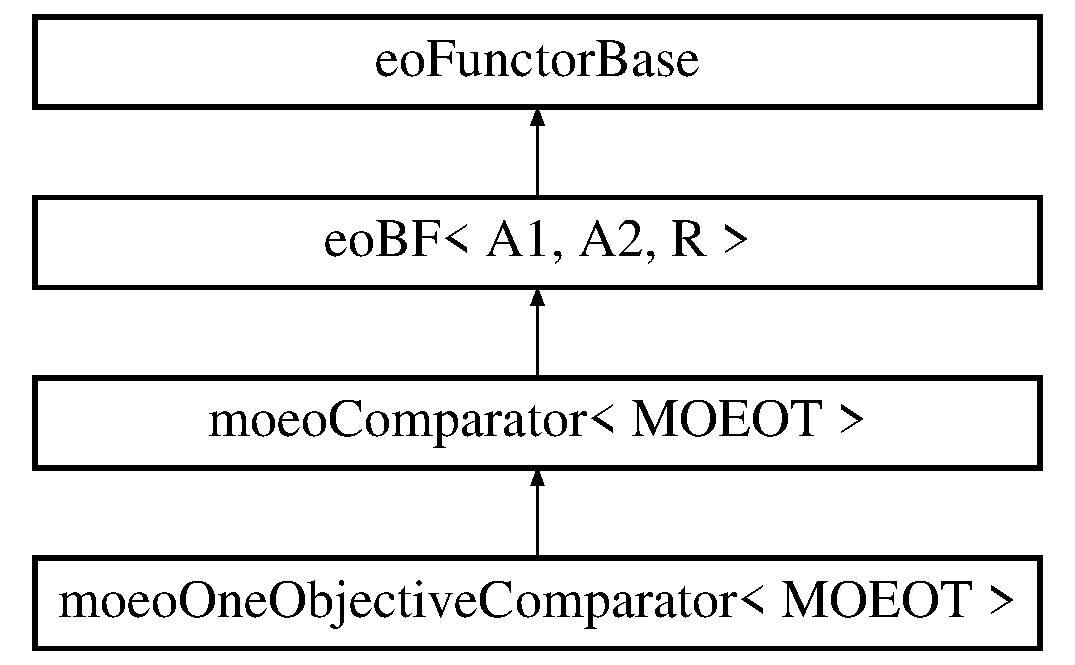
\includegraphics[height=4cm]{classmoeoOneObjectiveComparator}
\end{center}
\end{figure}
\subsection*{Public Member Functions}
\begin{CompactItemize}
\item 
{\bf moeo\-One\-Objective\-Comparator} (unsigned \_\-obj)
\begin{CompactList}\small\item\em Ctor. \item\end{CompactList}\item 
const bool {\bf operator()} (const MOEOT \&\_\-moeo1, const MOEOT \&\_\-moeo2)
\begin{CompactList}\small\item\em Returns true if \_\-moeo1 is greater than \_\-moeo2 on the obj objective. \item\end{CompactList}\end{CompactItemize}
\subsection*{Private Attributes}
\begin{CompactItemize}
\item 
unsigned {\bf obj}\label{classmoeoOneObjectiveComparator_210e1300281084eb5f9dd378e6ac5a32}

\begin{CompactList}\small\item\em the index of objective \item\end{CompactList}\end{CompactItemize}


\subsection{Detailed Description}
\subsubsection*{template$<$class MOEOT$>$ class moeo\-One\-Objective\-Comparator$<$ MOEOT $>$}

Functor allowing to compare two solutions according to one objective. 



Definition at line 48 of file moeo\-Comparator.h.

\subsection{Constructor \& Destructor Documentation}
\index{moeoOneObjectiveComparator@{moeo\-One\-Objective\-Comparator}!moeoOneObjectiveComparator@{moeoOneObjectiveComparator}}
\index{moeoOneObjectiveComparator@{moeoOneObjectiveComparator}!moeoOneObjectiveComparator@{moeo\-One\-Objective\-Comparator}}
\subsubsection{\setlength{\rightskip}{0pt plus 5cm}template$<$class MOEOT$>$ {\bf moeo\-One\-Objective\-Comparator}$<$ MOEOT $>$::{\bf moeo\-One\-Objective\-Comparator} (unsigned {\em \_\-obj})\hspace{0.3cm}{\tt  [inline]}}\label{classmoeoOneObjectiveComparator_5b8b31285c72a6fd17eba4e3ce0317fd}


Ctor. 

\begin{Desc}
\item[Parameters:]
\begin{description}
\item[{\em \_\-obj}]the index of objective \end{description}
\end{Desc}


Definition at line 56 of file moeo\-Comparator.h.

References moeo\-One\-Objective\-Comparator$<$ MOEOT $>$::obj.

\subsection{Member Function Documentation}
\index{moeoOneObjectiveComparator@{moeo\-One\-Objective\-Comparator}!operator()@{operator()}}
\index{operator()@{operator()}!moeoOneObjectiveComparator@{moeo\-One\-Objective\-Comparator}}
\subsubsection{\setlength{\rightskip}{0pt plus 5cm}template$<$class MOEOT$>$ const bool {\bf moeo\-One\-Objective\-Comparator}$<$ MOEOT $>$::operator() (const MOEOT \& {\em \_\-moeo1}, const MOEOT \& {\em \_\-moeo2})\hspace{0.3cm}{\tt  [inline]}}\label{classmoeoOneObjectiveComparator_962a4cbc308c30a83c9c485a79374f6a}


Returns true if \_\-moeo1 is greater than \_\-moeo2 on the obj objective. 

\begin{Desc}
\item[Parameters:]
\begin{description}
\item[{\em \_\-moeo1}]the first solution \item[{\em \_\-moeo2}]the second solution \end{description}
\end{Desc}


Definition at line 69 of file moeo\-Comparator.h.

References moeo\-One\-Objective\-Comparator$<$ MOEOT $>$::obj.

The documentation for this class was generated from the following file:\begin{CompactItemize}
\item 
moeo\-Comparator.h\end{CompactItemize}
